%%%%%%%%%%%%%%%%%%%%%%% file typeinst.tex %%%%%%%%%%%%%%%%%%%%%%%%%
%
% This is the LaTeX source for the instructions to authors using
% the LaTeX document class 'llncs.cls' for contributions to
% the Lecture Notes in Computer Sciences series.
% http://www.springer.com/lncs       Springer Heidelberg 2006/05/04
%
% It may be used as a template for your own input - copy it
% to a new file with a new name and use it as the basis
% for your article.
%
% NB: the document class 'llncs' has its own and detailed documentation, see
% ftp://ftp.springer.de/data/pubftp/pub/tex/latex/llncs/latex2e/llncsdoc.pdf
%
%%%%%%%%%%%%%%%%%%%%%%%%%%%%%%%%%%%%%%%%%%%%%%%%%%%%%%%%%%%%%%%%%%%

\documentclass[runningheads,a4paper]{llncs}

\usepackage{amssymb}
\setcounter{tocdepth}{3}

%% Use this for standard eps graphics, if it works for you adhoc
\usepackage{graphicx}
\usepackage{booktabs}
\usepackage{aicescover}

%% Use this for eps convertion to pdf.
%\usepackage[pdftex]{graphicx}
%\usepackage{epstopdf}

%Sprache und Links
\usepackage{url}
\usepackage{lscape}
\usepackage[utf8]{inputenc}
\usepackage[T1]{fontenc}
\usepackage[english]{babel}

%%%% HIER BITTE DIE EMAILADRESSEN EINTRAGEN
\urldef{\mails}\path|vitor.zago@rwth-aachen.de|
\newcommand{\keywords}[1]{\par\addvspace\baselineskip
\noindent\keywordname\enspace\ignorespaces#1}
\begin{document}
\aicescoverpage

\mainmatter  % start of an individual contribution
% first the title is needed
\title{Titel der Hausarbeit}

% a short form should be given in case it is too long for the running head
\titlerunning{Titel der Hausarbeit}


\author{Vitor Hugo Bellotto Zago}
\authorrunning{Bellotto Zago, Vitor Hugo}
% (feature abused for this document to repeat the title also on left hand pages)

% the affiliations are given next; don't give your e-mail address
% unless you accept that it will be published
\institute{
RWTH Aachen University, Germany\\
Enrollment number: 330110
\mails\smallskip
}
%
% NB: a more complex sample for affiliations and the mapping to the
% corresponding authors can be found in the file "llncs.dem"
% (search for the string "\mainmatter" where a contribution starts).
% "llncs.dem" accompanies the document class "llncs.cls".
%


\maketitle


\begin{abstract}

Englisches Abstract (150 Wörter). Eine Zusammenfassung der gesamten Arbeit. 
Inklusive Motivation, Stand der Forschung, Methode, Ergebnissen, und Diskussion.
Was nimmt man mit! Kein "Teasern".


\keywords{5 Schlüsselwörter}
\end{abstract}


%%%
%%% ACHTUNG! ACHTUNG! ACHTUNG! ACHTUNG! ACHTUNG! ACHTUNG!
%%%
%%% Das eigentliche Dokument ist in der Datei "text.tex"
% !TEX root = main.tex

%%%%
%%%% 1. INTRODUCTION
%%%%
\section{Introduction}
Motivation des Forschungsthemas aus der Literatur. Warum ist die Frage auf die man jetzt hinarbeitet von Bedeutung? Hier darf "geteasert" werden.


Interest in Computational Science. Subtopics:

\begin{itemize}
\item Mathematical
	\begin{itemize}
		\item Ito Calculus. Use of stochastic differential equation. Brownian motion.
		\item Monte Carlo Simulation
	\end{itemize}
	\item Finances
	\begin{itemize}
		\item Greeks
		\item LIBOR market.
	\end{itemize}
	\item Mathematical and Computational
	\begin{itemize}
		\item Finite Differences. $F'(x)$ at $O(n).Cost(F)$
	    \item Forward Method - Tangent Linear. $F'(x)$ at $O(n).Cost(F)$. 
	    \begin{equation}
	    	\frac{Cost(\dot{F})}{Cost(F)} \approx 2
	    \end{equation}
    	\item Reverse Method - Adjoint Method. $F'(x)$ at $O(m).Cost(F)$.
    	 \begin{equation}
	    	\frac{Cost(\dot{F})}{Cost(F)} < 30
	    \end{equation}
	\end{itemize}
	Source: %https://www.youtube.com/watch?v=F3wSYr_6fdU&t=926s
    


    
%% The computational efficiency was improved by a factor of 10 when the forward method was emplyed instead of finite differences. Then the adjoint approach reduced the cost by several orders of magnitude , compared to the forward appproach.	

\end{itemize}





%%%%%%%%%%%%%%%%%%%%%%%%%%%%%%%%%%%%%%%%%%%%%%%%%%%%%%%%%%%%%%%%%%%%%%%%%%%%%%%%%%%%%%%%%%%%%%%%%%%%%%%%%%%%%%%%
%%%%
%%%% 2. RELATED WORK
%%%%
\section{Motivation}

[ Comparison of \textit{finite differences}, \textit{forward method} and \textit{adjoint method}

The adjoint method produces exactly the same value on each simulated path as would be obtained using a forward implementation of the path wise method, but working backward along each path. It outperforms the forward implementation whenever the problem is to compulate the sensitivity of a small number of outputs to a large number of inputs. [PAPER1]

Advantages of adjoint method:
\begin{itemize}
\item The adjoint relation is a vector recursion whereas original formulas use a matrix rescursion. Hence, the adjoint has only to update the adjoint variables V(n) m times and the orginal algorithm has to update $m^2$ variables each time. [PAPER1]
\item According to the Algorithmic Differentiation, provided that the computational complexity of the adjoint calculation is no more than 4 times greater than the complexity of the orginal algorithm, the adjoint method will always be more efficient.
\end{itemize}

Drawbacks of the adjoint method:
\begin{itemize}
\item Pathwise approach is not applicable when the financial payoff function is not differentiable.
\item Execution of adjoint model is more expensive than the tangent model.
\end{itemize}


\section{Finances}
\subsection{LIBOR model market}
\subsection{Greeks}
\subsection{Monte Carlo simulation}

\subsection{Finite Differences}
Cost:?
\subsection{Forward Method}
Cost:?
\subsection{Adjoint method}
For a function $F:{\rm I\!R}^m \rightarrow {\rm I\!R}^n$, the first adjoint model is:
\begin{equation}
	x_{(1)}={\left(\frac{\partial F}{\partial x}{}\right)}^T y_{(1)} = J^T y
\end{equation}


\begin{equation}
  dX(t) = a(X(t))dt + b(X(t))dW(t)
\end{equation}






\subsection{Research question and hyphothesis}
How effective the adjoint method is in comparison with the finite method?
Welche Frage untersuche ich? Welche Hypothesen haben ich?
\begin{itemize}
\item \textbf{H1}: Große Menschen haben größere Füße.
\item \textbf{H2}: Große Menschen wiegen mehr als kleinere Menschen.
\end{itemize}



%%%%%%%%%%%%%%%%%%%%%%%%%%%%%%%%%%%%%%%%%%%%%%%%%%%%%%%%%%%%%%%%%%%%%%%%%%%%%%%%%%%%%%%%%%%%%%%%%%%%%%%%%%%%%%%%
%%%%
%%%% 3. METHODE
%%%%
\section{Method}


Der Methodenteil ist eine objektive Beschreibung des Vorgehens. Er ermöglicht es anderen Personen, die Forschung zu prüfen und somit zu validieren oder zu falsifizieren.

Die Methode beschreibt dabei sowohl das Vorgehen in der Erhebung (Prozedere) als auch das Vorgehen in der Auswertung (Statistik). 
Typischerweise wird hier auch der Fragebogen beschrieben und UV und AV benannt.









%%%%%%%%%%%%%%%%%%%%%%%%%%%%%%%%%%%%%%%%%%%%%%%%%%%%%%%%%%%%%%%%%%%%%%%%%%%%%%%%%%%%%%%%%%%%%%%%%%%%%%%%%%%%%%%%
%%%%
%%%% 4. RESULTS
%%%%
\section{Results}
Der Ergebnisteil beschreibt die relevanten Ergebnisse so kurz wie möglich und so lang wie nötig. Hierbei werden quantitative Ergebnisse nur berichtet und \textit{nicht} interpretiert.
Typischerweise beginnt man den Ergebnisteil mit der Beschreibung der Stichprobe.

\subsection{Beschreibung der Stichprobe}
Wieviele Probanden, etc.

\subsection{Deskriptive Statistik}
Beispielhaft blabla.



\subsection{Fragestellung ABC}
Beispielhaft blabla







%%%%%%%%%%%%%%%%%%%%%%%%%%%%%%%%%%%%%%%%%%%%%%%%%%%%%%%%%%%%%%%%%%%%%%%%%%%%%%%%%%%%%%%%%%%%%%%%%%%%%%%%%%%%%%%%
%%%%
%%%% 5. DISCUSSION
%%%%
\section{Diskussion}
In der Diskussion werden die Ergebnisse mit den Forschungsfragen und den Hypothesen zueinander in Beziehung gesetzt. Hierbei geht es nicht um eine Stellungnahme oder einen Kommentar, sondern um eine möglichst objektive Auseinandersetzung mit den Ergebnissen.

Die Ergebnisse sollen hierbei auch mit der Motivation (Kapitel 1) evaluiert werden. Was bedeuten diese Ergebnisse für die Wissenschaft?




\subsection{Limitationen und zukünftige Arbeiten}
Welche Einschränkungen müssen bei der aktuellen Arbeit berücksichtigt werden. Was hätte man anders machen sollen? Was konnte man nicht anders machen.

Wo ist der natürlich Anknüpfungspunkt für die nächsten Schritte.




%% ALLES HINTER DIESEM KOMMENTAR KANN GELÖSCHT WERDEN %%%
\newpage
\section{Beispiele}
Dieses Kapitel enthält Beispiele wie Bilder, Tabellen und Fußnoten verwendet werden können.

\subsection{Fußnote mit Link}

The website \textit{Google}\footnote{\url{https://www.google.com}} is a search engine. 


\subsection{Referenz auf Bild}
Bilder können gut benutzt werden um das Forschungsmodell zu zeigen (vgl. Abb. \ref{fig:researchmodel}).

%%%%%%% IMAGE %%%%%%%%%%% 
% Hier ist die Breite 0.7 gewählt entspricht 70% der Textbreite
\begin{figure}[htbp]
\centering
  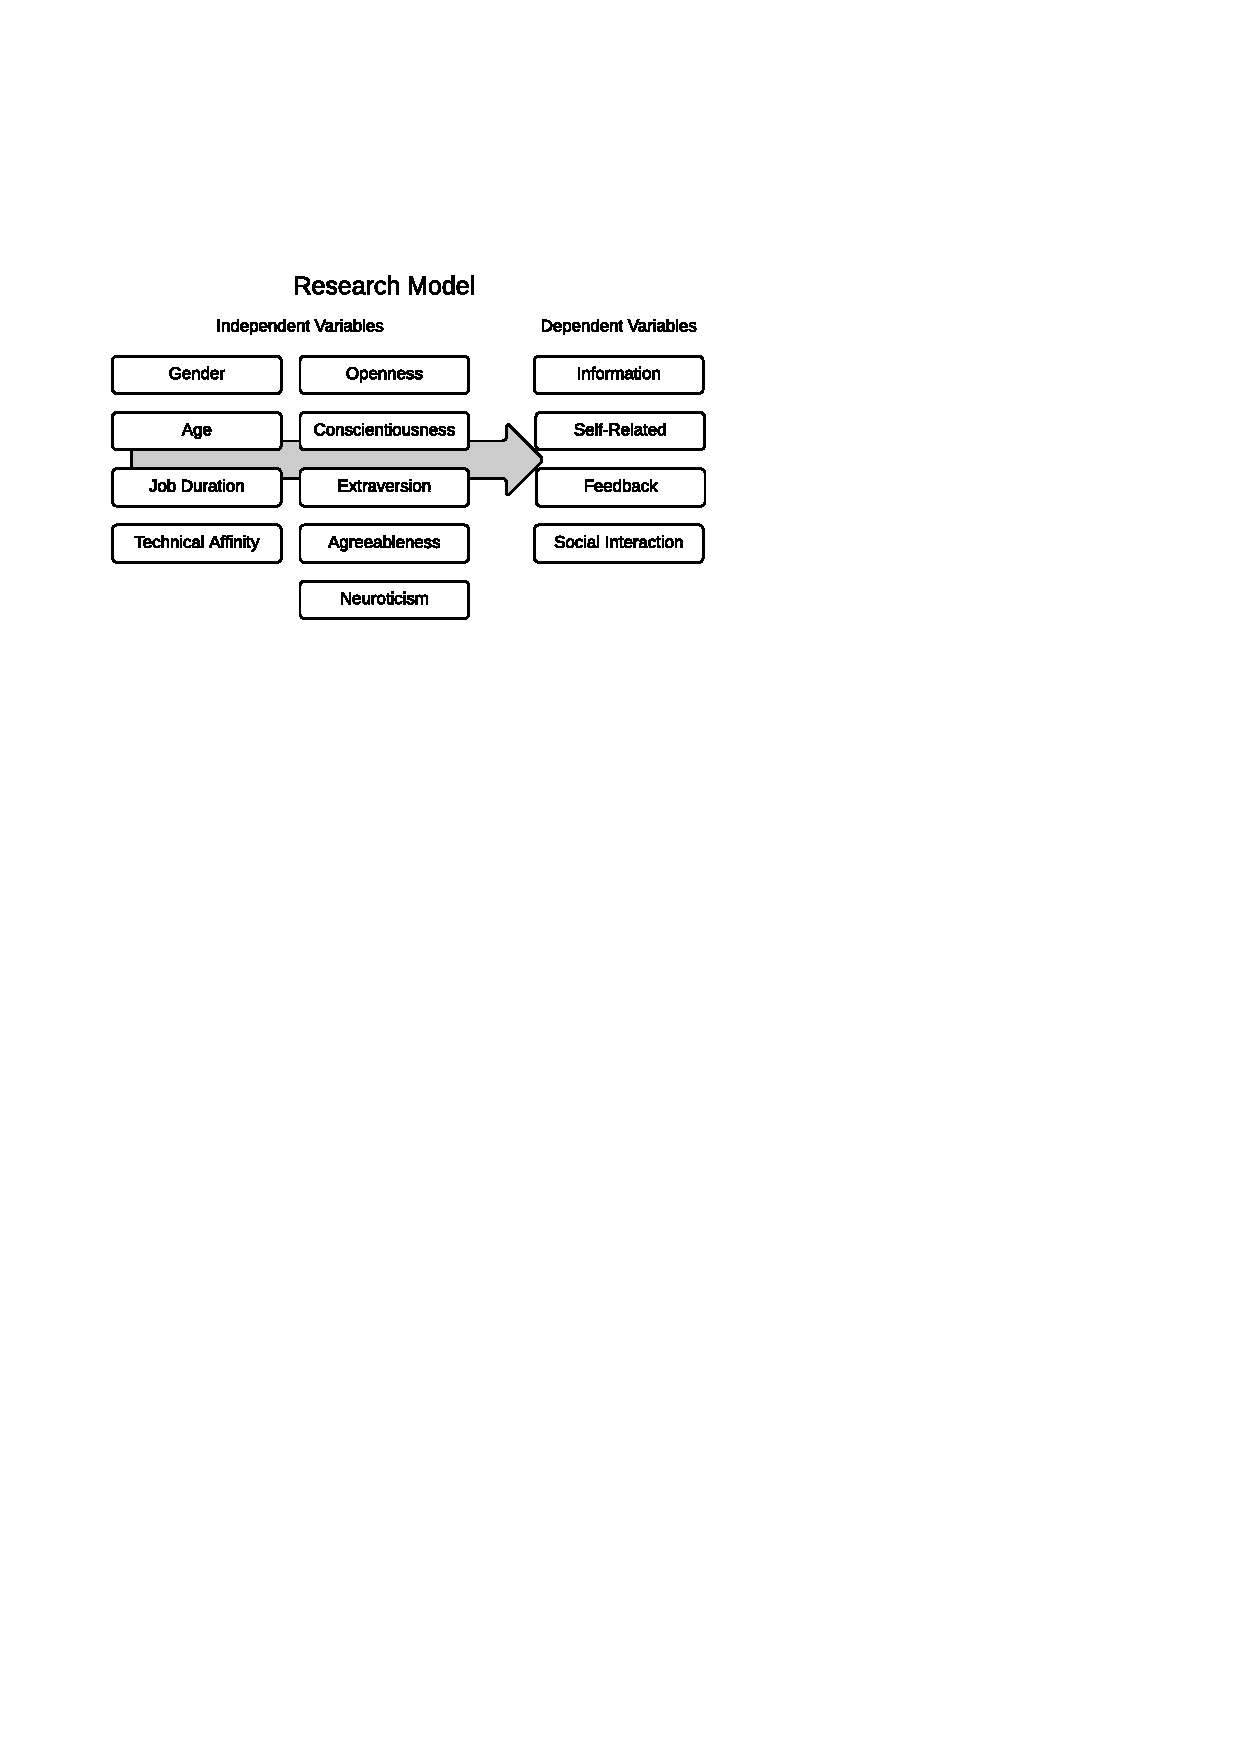
\includegraphics[width=0.7\textwidth]{researchmodel.pdf}
   \caption{Our case study investigating explanations for differences in usage motivation.}
\label{fig:researchmodel}
\end{figure}
%%%%%%% IMAGE %%%%%%%%%%%

\subsection{Beispiel Tabelle}


%%%%% TABELLE %%%%%%%%%
\begin{table}[htbp]
\centering
	\begin{tabular}{p{7.7cm}p{0.5cm}cc}
	\toprule
	\textbf{I use the software because,...} &	&	\textbf{Scale} & Loading\\
	\midrule 
    %I use the software because,...	& & \\
    I can access information more easily. & & Information & .825\\
    I can access information that is relevant for me.& & Information  & .817\\
    I will get informed about activities in my department. & & Information & .775 \\
    I can present my ideas. & & Information & .697 \\
	\bottomrule \\
\end{tabular}
\caption{Dependent variables: Item texts and scales. Loading refers to the factor-loading of the principal component analysis after varimax rotation with Kaiser-Normalization.}
\label{tab:ScalesMotives}
\end{table}
%%%%% TABELLE %%%%%%%%%

\subsection{Referenzen}
The usage of social networking sites (SNS) for business purposes seems to be a promising approach for enhanced connectivity and communication among employees independent from space, time and position \cite{dimicco2008motivations}. Since social media services like Facebook, Twitter and other SNS are part of our daily private lives \cite{stocker2013exploring}, their implementation as a business support tool spread with amazing rapidity \cite{koch2009enterprise}. 

Die Referenzen finden sich in der Datei: references.bib.







\bibliographystyle{splncs}
\makeatletter
\renewcommand\@biblabel[1]{#1. }
\makeatother
%----------------------------------------------------------
% Use the following option to include external BibTeX files:
\bibliography{references}

\end{document}

